% !TEX encoding = UTF-8 Unicode
\documentclass[11pt,a4paper]{report}
%\usepackage[a4paper, margin=20mm]{geometry}



\usepackage[utf8]{inputenc} 
%\usepackage[T1]{fontenc}
%\usepackage[slovene]{babel}    % pravila za slovensko deljenje besed




\usepackage{pdfpages}

%\usepackage[numbers]{natbib}


%%%%%%%%%%%%%%%%%%%%%%%%
% MATEMATIKA IN FIZIKA %
%%%%%%%%%%%%%%%%%%%%%%%%
% za matematiko
\usepackage{amsmath, amsfonts, xfrac, amssymb, mathrsfs, amsthm, bm, cuted}
% za enote
% \si{enota}
% \SI{cifra}{enota}
% \num{cifra}
% \ang{kot}
\usepackage{siunitx}
% Declare new unit
\DeclareSIUnit{\cal}{cal}
\DeclareSIUnit{\kcal}{\kilo\cal}
\DeclareSIUnit{\joul}{\J}
\DeclareSIUnit{\kjoul}{\kJ}
\DeclareSIUnit{\min}{\minute}
%\sisetup{output-decimal-marker = {,}}
\sisetup{separate-uncertainty=true,multi-part-units=single}
\sisetup{range-phrase = --}
%\sisetup{per-mode=reciprocal}
%\sisetup{group-separator = {.}}
% za uporabljanje decimalne vejice in ne pike
% pises decimalno piko, vendar ti zgenerira kot decimalno vejico
% to zato, da ko uporabljas vejico imas za vejico avtomatsko presledek
%\DeclareMathSymbol{.}{\mathord}{letters}{"3B}
% lahko bi uporabil tudi novo komando
\newcommand{\vejica}{{,}}
% lahko pa uporabljas \num{stevilka}, iz paketa siunitx

% za (1-3) pri enačbah
%\usepackage{cleveref}
\usepackage{eurosym}

%%%%%%%%%%%%%%%%%%%%%%%%%%%%%%
% TABELE IN SLIKE NASTEVANJE %
%%%%%%%%%%%%%%%%%%%%%%%%%%%%%%
%
% for adding tables that can span across multiple columns
\usepackage{xtab}
% za uporabo toprule bottomrule midrule za boljse tabele
\usepackage{booktabs} 
\usepackage[]{multirow}
% za align-annje na decimalni vejici
\usepackage{dcolumn}
% USAGE: ...\begin{tabular}{l r c D{separator in tex file}{ separator in output}{decimal places}}
% ovveride in heading with \multicolumn{1}{..}{..}

% za tabele katerim dolocimo širino in X specifier -> ta naredi stolpec tako
% dolg, da bo tabela zavzela določeno širino.
\usepackage{tabularx}
% ovveride in heading with \multicolumn{1}{..}{..}
\usepackage{etoolbox}
%\robustify\bfseries
\usepackage{longtable}

% za dodajanje slik
\usepackage{graphicx}
\graphicspath{{./pics/}}
\usepackage{epstopdf}
\usepackage{caption}
\usepackage{subcaption}

% Za dodajanje okvirjev okoli slik
\usepackage[export]{adjustbox}
% USAGE: 
% \includegraphics[<other options>, frame]{image}
% or
% \includegraphics[<other options>, fbox]{image}

% za tikz slikce
\usepackage{pgfplots}
\pgfplotsset{compat=1.12}
\usepgfplotslibrary{polar}
\pgfplotsset{plot style/.style={axis x line=middle, axis y line=
middle, xlabel={$x$}, ylabel={$y$}, axis equal }}

\pgfplotsset{polar plot style/.style = {
xticklabels={,,
$\frac{\pi}{6}$, $\frac{\pi}{3}$, $\frac{\pi}{2}$, $\frac{2\pi}{3}$,
$\frac{5\pi}{6}$, $\pi$, $\frac{7\pi}{6}$, $\frac{4\pi}{3}$,
$\frac{3\pi}{2}$, $\frac{5\pi}{3}$,$\frac{11\pi}{6}$,}, thick
}}

\pgfplotsset{hoof plot style/.style = {
polar plot style,
xtick={0,30,60,90,120,150,180,210,240,270,300,330},
xticklabels={$3$, $4$, $5$, $6$, $5$, $4$, $3$, $2$, $1$,, $1$, $2$}
}}

\usepackage{circuitikz, tikz, tikz-3dplot}
\usetikzlibrary{arrows, shapes, positioning, intersections, calc, shadings}
\usetikzlibrary{3d}
\newcommand{\blokec}[2]{node[draw, text centered, minimum width=4cm, minimum height=1cm, rounded corners, text width= 3cm, scale=1](#1){#2}}
    
\tikzset{dash/.style = {dashed, draw=black!50}}
\tikzset{dot/.style = {dotted, draw=black!50}}
\tikzset{base-axis/.style = {very thick}}
\tikzset{axis/.style = {base-axis, ->, >=stealth}}
\tikzset{plane/.style = {
	fill=teal!20, opacity=0.8,
    draw=teal!50!black!50,
    solid, thick
    }}
      
\tikzset{vec/.style = {->, >=stealth, solid, thick}}

\tikzset{velocity/.style = { vec, draw=orange!50!black!90}}


\tikzset{rect/.style = {
  rectangle,
  very thick, solid, rounded corners=1mm,
  top color=white,
  text centered, align=center,
  scale = 0.7
  }}
  \tikzset{title/.style = {
  % Rectangle:
  rect,
  draw=red!50!black!50,
  bottom color=red!50!black!20,
  % Text:
  text width = 30mm
  }}
  \tikzset{block/.style = {
  % Rectangle:
  rect,
  draw=black!50,
  bottom color=black!20
  % Text
  }}
  \tikzset{input/.style = {
  % Rectangle:
  block,
  draw=green!50!black!50,
  bottom color=green!50!black!20
  % Text
  }}
  \tikzset{output/.style = {
  % Rectangle:
  block,
  draw=orange!50!black!50,
  bottom color=orange!50!black!20
  % Text
  }}
  \tikzset{background/.style = {
  fill=black!10, 
  rounded corners, 
  draw=black!50, 
  dashed
  }}
  \tikzset{arrow/.style = {
  ->,
  >=stealth,
  shorten >= 1mm,
  shorten <= 1mm,
  very thick,
  draw=black!50,
  line width = 1mm
  }}
  \tikzset{angle/.style={
	fill=#1!20, opacity=0.8,
	draw=#1!50!black!50
	}}
  \tikzset{zxplane/.style={canvas is zx plane at y=#1}}
  \tikzset{yxplane/.style={canvas is yx plane at z=#1}}
  \newcommand{\spherical}[3]{xyz spherical cs:radius=#1,longitude=#3,latitude=#2}
  \newcommand{\cylindrical}[3]{xyz cylindrical cs:radius=#1,z=#3,angle=#2}
  

% za odštevanje pri listih
%\usepackage[start=7]{etaremune}
% za seznam kjer lahko spreminjaš številke
% dodati moraš [label = nekaj]
% če hočeš številke dodaš \arabic*
% če hočeš črke dodaš \alph* ali \Alph*
% če hočeš rimske številke dodaš \roman* ali \Roman*
\usepackage{enumitem}
% za listo v dveh stolpcih
\usepackage{multicol}
% za dodajanje besedila iz drugih datotek
\usepackage{verbatim}
% za urlje 
%\usepackage[unicode, hidelinks]{hyperref}
\usepackage{hyperref}
\hypersetup{hidelinks}
\usepackage{bookmark}
\usepackage{fancyhdr}


%\usepackage[style=ieee]{biblatex}
%%%%%%%%%%%%%%%%
% NOVE KOMANDE %
%%%%%%%%%%%%%%%%
\usepackage{xspace} % da latex dojame da mora dat presledke med komandami
\newcommand{\stopinj}{^\circ}
\newcommand{\sintaksa}[1]{\xspace``\texttt{#1}''\xspace}
\newcommand{\modd}{\uppercase{modd}\xspace}
\newcommand{\opencv}{OpenCV\xspace}


\newcommand{{\T}}{\ensuremath{^{\top}}}
\newcommand{\Mu}{M}
\renewcommand{\Xi}{X}
\newcommand{\norm}[1]{\left\lVert #1 \right\rVert}
\renewcommand{\vec}[1]{{\ensuremath{\boldsymbol{#1}}\xspace}}

\newcommand{\esvr}{\ensuremath{\epsilon}-SVR\xspace}
\newcommand{\nusvr}{\ensuremath{\nu}-SVR\xspace}

\newcommand{\corr}{{CORR}\xspace}
\newcommand{\rmse}{{RMSE}\xspace}
\newcommand{\rae}{{RAE}\xspace}
\newcommand{\rrse}{{RRSE}\xspace}

\newcommand{\proc}[1]{\SI{#1}{\%}\xspace}

\newcommand{\boldentry}[3]{%
  \multicolumn{1}{S[table-format=#1.#2,
				  	round-mode=places, round-precision=#2,
                    mode=text,
                    text-rm=\fontseries{b}\selectfont
                   ]}{#3}}
\newcommand{\thead}[1]{\multicolumn{1}{c}{\textbf{#1}}}
\newcommand{\theadc}[1]{\multicolumn{2}{c}{\textbf{#1}}}
\newcommand{\theadm}[1]{\thead{\ensuremath{\mathbf{#1}}}}
\newcommand{\tdata}[1]{\input{./tab/#1.tex}}

\newcommand{\rnum}[1]{\romannumeral #1 \xspace}
\newcommand{\Rnum}[1]{\MakeUppercase{\rnum{#1}}}

\newcommand{\folder}{./section}

\let\originalcite\cite
\renewcommand{\cite}[1]{\unskip~\originalcite{#1}}
\let\originalref\ref
\renewcommand{\ref}[1]{\unskip~\originalref{#1}}

\usepackage{thmtools}
\declaretheoremstyle[
spaceabove=6pt, spacebelow=6pt,
headfont=\normalfont\bfseries,
notefont=\mdseries, notebraces={(}{)},
bodyfont=\normalfont,
postheadspace=0.6em,
headpunct=:
]{mystyle}
\declaretheorem[style=mystyle, name=Hipoteza, preheadhook={\renewcommand{\thehyp}{H\textsubscript{\arabic{hyp}}}}]{hyp}






%\usepackage{vmargin}
%\setmarginsrb{3 cm}{2.5 cm}{3 cm}{2.5 cm}{1 cm}{1.5 cm}{1 cm}{1.5 cm}

\title{Related work}                             % Title
\author{Gregor Koporec, mag. inž. el.}                               % Author
\date{\today}                                           % Date

\makeatletter
\let\thetitle\@title
\let\theauthor\@author
\let\thedate\@date
\makeatother

\pagestyle{fancy}
\fancyhf{}
\rhead{\theauthor}
\lhead{\thetitle}
\cfoot{\thepage}


\usepackage[backend=biber, style=ieee]{biblatex}
\def\citea#1{\citeauthor*{#1} \cite{#1}\xspace}
\addbibresource{./related.bib}
\addbibresource{./dataset.bib}
\addbibresource{./images.bib}
\addbibresource{./other.bib}

\begin{document}
%%%%%%%%%%%%%%%%%%%%%%%%%%%%%%%%%%%%%%%%%%%%%%%%%%%%%%%%%%%%%%%%%%%%%%%%%%%%%%%%%%%%%%%%%

\begin{titlepage}
	\centering
	\vspace*{0.2 cm}
	\includegraphics[width = 0.5\columnwidth]{logo}\\[1.0 cm]   % University Logo
	%\textsc{\LARGE Univerza v Ljubljani}\\[2.0 cm]   % University Name
	%\textsc{\Large Course Code}\\[0.5 cm]               % Course Code
	\textsc{\large PhD Thesis}\\[0.5 cm]               % Course Name
	\rule{\linewidth}{0.2 mm} \\[0.4 cm]
	{ \huge \bfseries \thetitle}\\
	\rule{\linewidth}{0.2 mm} \\[1.5 cm]
	
	\begin{minipage}{0.4\textwidth}
		\begin{flushleft} \large
			\emph{Author:}\\
			\theauthor
		\end{flushleft}
	\end{minipage}~
	\begin{minipage}{0.4\textwidth}
		\begin{flushright} \large
			\emph{Menthor:} \\
			prof. dr. Janez Perš                                   % Your Student Number
		\end{flushright}
	\end{minipage}\\[2 cm]
	
	{\large \thedate}\\[2 cm]
	
	\vfill
	
\end{titlepage}

%%%%%%%%%%%%%%%%%%%%%%%%%%%%%%%%%%%%%%%%%%%%%%%%%%%%%%%%%%%%%%%%%%%%%%%%%%%%%%%%%%%%%%%%%

\tableofcontents
%\pagebreakGauss

%%%%%%%%%%%%%%%%%%%%%%%%%%%%%%%%%%%%%%%%%%%%%%%%%%%%%%%%%%%%%%%%%%%%%%%%%%%%%%%%%%%%%%%%%

	%\thispagestyle{empty}
	\chapter{Podobna dela}
Globoke nevronske mreže močno vplivajo na raziskave v računalniškem vidu in strojnem učenju, saj po zmogljivostnih testih premagujejo večino algoritmov, ki jih je razvil človek \cite{sunderhauf2018the}. Zavedati se moramo, da imajo kljub temu DNN pomankljivosti, zato velikokrat odpovejo v realističnem okolju~\cite{sunderhauf2018the}. Glavni poudarek, zakaj prihaja do razlik med zmogljivostnimi testi na podatkovnih bazah in realnim okoljem je, da se pri zmogljivostnih testih raziskovalci osredotočajo na evaluacijske statistike, ki povzemajo zmogljivost algoritmov \cite{sunderhauf2018the}. Kot je poudaril \citea{sunderhauf2018the}: ``Če statistika govori, da je bila podatkovna baza rešena, še ne pomeni, da je bil problem rešen." Trditve, da so nevronske mreže presegle človeško zmogljivost, temeljijo na zmogljivostnih testih in so napačne ter zavajujoče. Pri primerjanju zmogljivosti z ljudmi bi potrebovali drugačen pristop, kot je vizualna psihofizika, ki je predstavljena v nadaljevanju. 


Nadaljnje, podatkovne baze ne povzemajo naravnih scenarijov, saj so te zgrajene na slikah in video posnetkih iz interneta \cite{sunderhauf2018the}. Podatkovne baze vsebujejo inherentno pristranskost, ki vpliva na evaluacijo in interpretacijo rezultatov. Pristranskost je opisana v poglavju .


Nikakor ne razumemo, kako se nevronske mreže obnašajo v scenarijih, kjer se okolje dinamično spreminja in kjer se pojavljajo objekti nezananega razreda \cite{sunderhauf2018the}. Prav tako se lahko zgodi, da so objekti v realnem scenariju na videz drugačni kot so bili predstavljeni v učni množici. Raziskovalci so pokazali, da lahko že z manjšimi spremembami močno vplivamo na odločitve nevronske mreže. Eden izmed razlogov je ta, da se globoki modeli trenutno uporabljajo v zaprtih sistemih, kjer so razredi popolnoma znani \cite{sunderhauf2018the}. Nevronske mreže bi morali razviti v bolj fleksibilne strukture, ki bi imele možnost razširiti svoje znanje z majhnim številom podatkov \cite{sunderhauf2018the}. %Prav tako bi morale znati oceniti negotovost rezultatov. Današnji sistemi preko softmax sloja vračajo zaupanje v predikicjo, ampak to niso kalibrirane verjetnosti.


\section{Primerjava med ljudmi in algoritmi}
\subsection{Vizualna izkrivljanja slike} \label{sec:psihofizika}
\citea{richardwebster2016psyphy} se je v svojem delu spraševal, če algoritmi razpoznavanja res delujejo tako dobro, kot mislimo. Glede na trenutno uporabljene statistike bi lahko verjeli, da smo dosegli človeško zmogljivost. Seveda pri tako veliki količini podatkov težko ugotovimo, kje algoritmi ne delujejo. Zato so avtorji predstavili novo metodo evaluacije, ki temelji na vizualni psihofiziki (angl. Visual Psychophysics). Pri tej metodi obravnavamo odnos med kontrolnim dražljajem in odzivom nanj. S perturbacijami izbranega dražljaja dobimo krivuljo odziva in jo uporabimo za primerjanje med modeli. 


\begin{figure}[!htbp]
	\centering
	\includegraphics[width=0.7\columnwidth]{richardwebster_1}
	\caption{Slike iz ImageNet podatkovne baze \cite{deng2009imagenet}.}
\end{figure}

V \cite{richardwebster2016psyphy} so najprej določili naključen niz slik za izbrano kategorijo. Iz niza so nato izluščili sliko s kanoničnim pogledom. Avtorji so nato perturbirali izbrane kanonične slike in jih uporabili pri testiranju razvrščanja. Za vsako kategorijo so na koncu dobili srednjo natančnost. Točke so interpolirali in zgladili pravokotnim oknom širine \num{15}. 

Kanonično sliko so v \cite{richardwebster2016psyphy} opredelili kot sliko, pri kateri dobimo največji odziv za privzeto vrednost dražljaja. Pri ljudjeh so to slike, kjer bo večina razpoznala objekt na sliki. Za modele kanonični pogled predstavlja sliko, kjer bo verjetnost razpoznavanja kategorije največja.

Testiranje razvrščanja so razdelili na dva testa. S prvim, \emph{2AFC}, so želeli preizkusiti razpoznavanje na temeljni ravni. Z drugim testom, \emph{MAFC}, pa so želeli preizkusiti rapoznavanje, ki je bolj primeren več razrednemu razvrščanju izbranih algoritmov. 

Pri 2AFC testu so najprej merjencu pokazali vzorčno sliko. Sledil je prikaz dveh alternativ, izmed katerih je ena pozitivna (iz iste kategorije) in druga negativna slika (iz različne kategorije). Merjenec je nato izmed alternativnih slik moral izbrati najbolj ugodno. Test so nato ponavljali za različne perturbacije kanoničnih slik. 

MAFC test so določili kot posplošeno obliko 2AFC testa. V tem testu so za vzorec izbrali vse slike, ki so jih uporabili pri učenju. Za altnernativne slike so izbrali kanonične slike iz vseh kategorij. Zaradi velikega števila slik, so pri tem testu subjektom primerno zmanjšali količino.

Perturbacijo slike je \citea{richardwebster2016psyphy} določil s popačitvami slike. Uporabil je Gaussovo glajenje, linearno okluzijo, šum sol in poper, osvetlitev, kontrast in ostrino.

Za podatkovno bazo slik so izbrali ImageNet 2012. Testirali so najbolj pogoste konvolucijske nevronske mreže AlexNet, CaffeNet, GoogleNet, VGG-16 in VGG-19. Študijo so izvedli s pomočjo 24 subjektov.

Ugotovili so, da natančnost modelov v vseh primerih začne hitro upadati pod \SI{80}{\%}. Ljudje so nevronske mreže prekašali v skoraj vseh testih. Največja razlika se je pojavila pri testiranju osvetlitve, kjer so bili ljudje za $\sim$\SI{9}{\%} slabši. 

Podobno nižjenivojsko primerjavo med modeli in ljudmi,  kot v \cite{richardwebster2016psyphy}, so predstavili v delu \cite{dodge2017a}. Test s subjekti so razdelili na tri dele. V prvem delu so merjenci videli primerke slik iz vseh izbranih kategorij. S tem so simulirali učenje nevronskih mrež. Sledil je korak validacije. Merjenci so razvrščali čiste slike. V primeru slabega razvrščanja so celoten test označili za osamelec. Tako so uporabili le rezultate merjencev, ki so test skrbno in resno izvedli. Nazadnje je sledil korak testiranja, kjer so merjenci razvrščali popačene slike. Slike so se na zaslonu pojavljale vedno od največje do najmanjše popačitve. S tem so se avtorji znebili efekta spomina, kjer bi lahko merjenec dopolnil manjkajočo informacijo s prejšnjim spoznanjem pri sliki z manjšim popačenjem. 

\begin{figure}[!htbp]
	\centering
	\includegraphics[width=0.7\columnwidth]{dodge_1}
	\caption{Slike iz ImageNet podatkovne baze \cite{deng2009imagenet}.}
\end{figure}

Za namen testiranja modelov so avtorji modelom dodali nov sloj za razvrščanje izbranih kategorij. Sloj so naučili z nepopačenimi slikami in ga še bolj natančno nastavili z dodatnim učenjem na popačenih slikah. Testiranje modelov je nato potekalo na enak način, kot pri subjektih.

Pri testiranju so \citea{dodge2017a} uporabili ImageNet podatkovno bazo. Zaradi velike količine podatkov, so izbrali le 10 kategorij. Vse kategorije so bile vrste psov. Izbiro kategorij avtorji zagovarjajo s tem, da so izbrane kategorije zelo povezane in tako težko ločljive. Za popačitev slike so uporabili Gaussov šum in glajenje. Rezultate na subjektih so dobili s $15$. merjenci. Za primerjavo so vzeli modele ResNet, GoogleNet in VGG-16. 

Z raziskavo so ugotovili, da je človeška natančnost večja od vseh modelov. Prav tako so poudarili, da ljudje hitreje izgubljajo na natačnosti pri meglenih slikah, modeli pa na pošumljenih slikah.

Skoraj identičen način eksperimentiranja sta avtorja iz \cite{dodge2017a} uporabila tudi v delu \cite{dodge2017can}, kjer sta testirala nižjenivojski človeški vidni sistem. Za razliko od \cite{dodge2017a} sta v \cite{dodge2017can} omejila opazovanje slike na \SI{100}{\ms}. Izbiro sta argumentirala s tem, da se v tako kratkem času oko ne premakne, zato je človekov vizualni sistem omejen na globalno reprezentacijo slike. Tudi v tem primeru sta ugotovila, da je človeška zmogljivost boljša od algoritmov.


Za razliko od ostalih so v \cite{geirhos2017comparing} teste na subjektih izvajali v kontroliranem laboratorijskem okolju, kjer so na zaslon najprej za \SI{300}{\ms} prikazali prazen okvir. Sledil je prikaz izbrane slike za \SI{200}{\ms}. Takoj zatem so merjencu prikazali masko šuma za \SI{200}{\ms}. Na koncu so imeli merjenci na voljo še \SI{1.5}{\s}, da so izbrali eno izmed ponujenih kategorij.

\begin{figure}[!htbp]
	\centering
	\includegraphics[width=0.7\columnwidth]{geirhos_1}
	\caption{Slike iz \cite{geirhos2017image} po licenci \url{https://creativecommons.org/licenses/by/4.0/legalcode}.}
\end{figure}

Pred samim testom so merjencem poakazali vse možne kategorije, da so zagotovili jasnost naloge. S prikazom maske šuma so minimizirali povratni vpliv v možganih, ker izbrani modeli nevroskih mrež ne vsebujejo povratnega vpliva.

Pri testiranju so \cite{geirhos2017comparing} uporabili ImageNet 2012 podatkovno bazo. Testirali so na $16$. kategorijah, ki so jih določili s pomočjo MS COCO podatkovne baze. Za popačenje so izbrali naslednje degradacijske metode: barva, kontrast, beli šum in eidolon. Eidolon je parametrično kontrolirana degradacija slike, ki povzroči podobno vizualno zavedanje na človeku \cite{geirhos2017comparing}. $3$ merjenci (moški, starost: 22--28 let, povprečje: 25 let) so sodelovali pri barvnem testiranju in po $5$ merjencev (6 moških in 4 ženske, starost: 19--28 let, povprečje: 23 let) je sodelovalo na ostalih testih. Za modele so izbrali AlexNet, GoogleNet in VGG-16. \citea{geirhos2017comparing} so ugotovili, da so CNN-ji manj robustni na popačenja slik kot ljudje.

Zelo podoben test, kot \cite{geirhos2017comparing}, so izvajali tudi v delu \cite{wichmann2017methods}. Tu so testirali DNN modele, če njihova zmogljivost degradira podobno kot človeška zmogljivost. V ta namen so primerjali DNN in ljudi pri spreminjanju kontrasta slike. Kontrast so izbrali zato, ker je relativno dobro razumljen vidik človeškega vida. Ker ljudje po navadi kategorizirajo slike po osnovnih kategorijah, so za testiranje uporabili MS COCO podatkovno bazo \cite{?}. Merjencem so vsako sliko pokazali za \SI{200}{\ms}. Sledil je prikaz roza šuma. Nazadnje so morali merjenci v roku \SI{1500}{\ms} izbrati eno izmed 16 kategorij.

\begin{figure}[!htbp]
	\centering
	\includegraphics[width=0.7\columnwidth]{wichmann_1}
	\caption{Slike iz \cite{geirhos2017image} po licenci \url{https://creativecommons.org/licenses/by/4.0/legalcode}.}
\end{figure}

Avtorji so s svojo raziskavo ugotovili, da AlexNet, GoogleNet in VGG-16 razpoznavajo polno kontrastne slike podobno kot ljudje. Podobnosti z zmanjševanjem kontrasta hitro izginejo, kar se opazi tako na krivulji natančnosti glede na kontrast kot tudi na konfuzijski matriki. Na podlagi konfuzijskih matrik so ugotovili, da DNN-ji vseeno niso dobri modeli človeškega ventralnega procesiranja, saj bi v nasprotnem primeru pričakovali, da oboji delajo podobne napake.


\subsection{Razlike v zornem kotu}
\citea{kheradpisheh2016deep} so preizkušali delovanje glede na pozicijo, velikost in orientacijo objektov. S tem so želeli ugotoviti, ali se nevronske mreže naučijo invariantnosti na izbrane parametre. Za testiranje so renderirali slike iz 3D računalniških modelov, kjer so za parametre 3D transformacij uporabljali naključno število. Modelom so dodajali tudi različna ozadja iz realnih slik. 

\begin{figure}[!htbp]
	\centering
	\includegraphics[width=0.7\columnwidth]{kheradpisheh_1}
	\caption{Slike naravnega ozadja so iz \cite{xiao2010sun}. 3D modeli so iz \cite{oreilly2013recurrent}. Slika kategorij je iz \cite{geirhos2017image} po licenci  \url{https://creativecommons.org/licenses/by/4.0/legalcode}.}
\end{figure}

Pri testiranju subjektov so uporabljali podobno metodologijo, kot \cite{geirhos2017comparing}. Prvih \SI{500}{\ms} so prikazovali črn križec ali naravno ozadje. Sledil je prikaz izbrane slike za \SI{25}{\ms} in nato prazen zaslon za enak časovni interval. Nato so prikazali masko šuma za \SI{100}{\ms} in na koncu še slike kategorij, izmed katerih so merjenci eno izbrali.  

Pri evaluaciji modelov so prednaučenim modelom podali naključno izbran niz učnih in testnih slik. Za vsako sliko so za vsak sloj modela dobili vektor značilk. Vektorje so nato uporabili za učenje in testiranje SVM razvrščevalnika. Tak način testiranja so $15\times$ ponovili za vse modele, sloje in vrednosti parametrov 3D transformacij. S tem so dobili povprečno vrednost in standardni odklon natančnosti delovanja modela in posameznih slojev modela za izbran parameter transformacije.

Za testiranje so uporabili že prej opisane renderirane slike z objekti iz $5$. različnih kategorij ($600$ slik na kategorijo). Vsak objekt so transformirali na $7$ različnih načinov, pri tem pa so uporabili po $2$ različna ozadja. Tako so dobili $14$ podatkovnih baz s $3000$ slikami. Testirali so $26$ subjektov ($17$ moških in $9$ žensk, starost $21$--$32$ let, povprečje starosti $26$ let) in $9$ različnih modelov nevronskih mrež.

V raziskavi so ugotovili, da delujejo modeli skoraj tako dobro kot ljudje, če imajo objekti enakomerno sivo ozadje. Pokazali so tudi, da dodajanje slojev v nevronskih mrežah poveča natančnost glede na parametre 3D transformacij. 

Z manjšimi spremembami so avtorji dela \cite{kheradpisheh2016deep} ponovili poskus v \cite{kheradpisheh2016humans}. Tu so razdelili podatkovno bazo na 3 dele. V vsakem delu so spreminjali izbrano število parametrov pozicije in rotacije. Prav tako so deloma spremenili psihofizioliške eksperimente, ki so bolj podrobno predstavljeni na sliki \ref{}. 

\begin{figure}[!htbp]
	\centering
	\includegraphics[width=0.7\columnwidth]{kheradpisheh_2}
	\caption{Slike naravnega ozadja so iz \cite{xiao2010sun}. 3D modeli so iz \cite{oreilly2013recurrent}. Slika kategorij je iz \cite{geirhos2017image} po licenci  \url{https://creativecommons.org/licenses/by/4.0/legalcode}.}
\end{figure}

V \cite{kheradpisheh2016humans} so raziskovalci ugotovili, da ljudje razpoznavajo objekte tudi pri velikih variacijah, so zelo natačni in imajo kratek odzivni čas. Natančnost in odzivni čas sta močno odvisna od tipa variacije. Raziskave so pokazale da je rotacija v globino najtežja. Za DNN-je so ugotovili, da so močno korelirani z ljudmi. Tudi nevroske mreže so imele težave pri rotaciji v globino. 



\subsection{Primerjava modelov, ki ne temeljijo na nevronskih mrežah}
\citea{borji2014human} so v svojem delu izvedli obsežno raziskavo primerjave med človeškim in računalniškim razpoznavanjem objektov in prizorov. Pri tem so uporabili $14$ modelov, $7$ podatkovnih baz in $5$ različnih testov. 

Prvi test so uporabili za preverjanje moči vizualnega razlikovanja in reprezentacije med ljudmi in algoritmi. V tem testu so preverjali kako dobro algoritmi in ljudje razlikujejo med različnimi prizori in če zaznajo razlike kaj je žival in kaj ni. Drugi test so namenili razpoznavanju črtnih slik (nizko nivojsko razpoznavanje). V tretjem testu so se osredotočili na analizo invariantnosti pri razpoznavanju tipa žival ne-žival. Pri tem so uporabili skaliranje in vrtenje v ravnini. Razpoznavanje lokalne in globalne informacije iz slik so testirali v četrtem testu. Tu so uporabili slike, kjer so njeni deli med seboj premešani. Zadnji test so uporabili za večrazredno razpoznavanje objektov na velikih podatkovnih bazah.

\begin{figure}[!htbp]
	\centering
	\includegraphics[width=0.7\columnwidth]{borji_1}
	\caption{Slike iz \cite{xiao2010sun} in \cite{griffin2007caltech}.}
\end{figure}

Za modele so izbrali enorazredne SVM razvrščevalnike z 10 kratno križno validacijo. Izbrani deskriptorji so temeljili na HOG in SIFT deskriptorjih in Gaborjevih filtrih za razpoznavanje prizorov. Natančnost modelov so izračunali kot povprečje konfuzijskih matrik za posamezno križno validacijo. 

Pri razikovanju so ugotovili da v prvem testu najmanj polovica algoritmov deluje z natančnostjo nad \SI{70}{\%} medtem ko je natančnost ljudi okoli \SI{80}{\%}. V manjši meri so algoritmi celo dosegali natančnost ljudi. V drugem testu so ljudje bili sposobni razpoznati prizor iz črtnih slik z natačnostjo \SI{66}{\%}, algoritmi pa z natančnostjo preko \SI{70}{\%}. Pri testiranju invariantnosti so ugotovili, da rotacija na ljudi zelo malo vpliva glede na algoritme. Na zmešanih slikah so se algoritmi večinoma bolje odrezali kot ljudje, kjer slike predstavljajo zunanji prizor in slabše na slikah z notranjim prizorom. Njihovo slabo delovanje za zmešane slike z objekti je nakazovalo, da modeli večinoma temeljijo na zbiranju globalne informacije iz slik. V zadnjem testu so raziskovalci ugotovili, da najboljši modeli ne dosegajo sposobnosti človeškega razpoznavanja. Razlika med njimi je bila okoli \SI{17}{\%}.

\subsection{Razvrščanje v abstraktne razrede}
Objekti različnih kategorij, okluzija in nepričakovane postavitve so tipični pojavi, pri katerih današnji algoritmi, glede na človeka, delujejo slabo \cite{fleuret2011comparing}. Za dobro delovanje pri tako veliki kompleksnosti avtorji iz \cite{fleuret2011comparing} zato zagovarjajo, da algoritmi potrebujejo neko vrsto globalnega presojanja, s katerim lahko zgradijo višjenivojske koncepte - abstrakcije. 

\begin{figure}[!htbp]
	\centering
	\includegraphics[width=0.7\columnwidth]{fleuret_1}
	\caption{}
\end{figure}

V ta namen so razvili kontroliran eksperiment, SVRT, s katerim bi lahko izmerili razliko v abstraktnem presojanju med ljudmi in algoritmi. Pri tem gre za serijo $23$ različnih problemov, ki vsebujejo slike z naključno generiranimi oblikami brez kakršnega koli pomena. S takim testom se znebimo problemov razvrščanja naravnih slik pri algoritmih, kot so osvetlitev, tekstura in šum. Prav tako zmanjšamo prednost človeka pred algoritmi, ker imajo veliko izkušenj z naravnimi objekti v 3D svetu \cite{fleuret2011comparing}. 

Vsak problem v SVRT je sestavljen iz dveh izključujočih razredov slik. Posamezen razred vsebuje abstraktno lastnost, ki ni vključena v drugem. Abstraktne lastnosti temeljijo samo na odnosih med oblikami.

Za testiranje subjektov so uporabili 20 ljudi (6 moških in 14 žensk, starost: 18--21). Merjencu so po vrsti prikazovali eno naključno sliko iz izbranega problema, ta pa jih je zlagal v eno ali drugo kategorijo. Po vsaki zložitvi je merjenec dobil odgovor o pravilnosti razvrščanja. Prav tako so bile na zaslonu prikazane vse pravilno razvrščene slike. S tem so merjencem pomagali pri dojemanju abstraktnih lastnosti. Za testiranje algoritmov so uporabili Adabost in SVM z Gaussovim jedrom.

S tovrstnim testiranjem so ugotovili, da ljudje za popolno razvrščanje rabijo manj kot $20$ slik za učenje medtem, ko se delovanje algoritmov izboljšuje z večanjem števila učnih slik nad \num{10000}. Več kot \SI{90}{\%} ljudi je rešilo 14 od 23 problemov medtem ko so algoritmi rešili le 11 problemov z napako razvrščanja pod \SI{10}{\%}.

Enak test so uporabili tudi \citea{stabinger201625}, s katerim so želeli ugotoviti kakšen napredek smo dosegli s CNN pri razvrščevanju slik v abstraktne kategorije. Primerjali so delovanje dveh konvolucijksih mrež GoogleNet in LeNet.  

S preprostim primerjanjem natančnosti so ugotovili, da v 25 letih ni bilo praktično nobene razlike. Povprečje obeh mrež je bila okoli \SI{77}{\%} (človek \SI{93}{\%}). Dodatno testiranje je pokazalo, da CNN niso sposobni reševati problemov primerjave oblik. Brez te primerjave je natančnost GoogleNet prekašala tako LeNet kot človeka. Seveda so pri tem poudarili, da CNN potrebuje vsaj $4000$ slik za učenje. 

Problem takega testiranja je, kot so že poudarili v \cite{fleuret2011comparing}, da ni prilagojen za otroke, ki še nimajo dovolj razvitega logičnega razmišljanja. Prav tako ni razvidno, kako poteka abstraktno dojemanje konceptov na naravnih slikah. Seveda je prav tako težko določiti ali se razvrščevalniki sploh naučijo abstraktnih lastnosti, ki jih podamo v testu.

\subsection{Sistematična razlika med modeli in ljudmi}
V \cite{pramod2016computational} se avtorji sprašujejo, če razlika med ljudmi in stroji obstaja zaradi sistematičnih razlik. V ta namen so uporabili primerjavo razdalj med objekti v prostoru značilk. 

\begin{figure}[!htbp]
	\centering
	\includegraphics[width=0.7\columnwidth]{pramod_1}
	\caption{Slike iz \cite{pramod2016computational}.}
\end{figure}


Podatkovno bazo so zgradili iz naravnih objektov in silhuet. Vse slike so vsebovale izolirane objekte, brez ozadja. Objekti so bili iz različnih kategorij kot so živali, orodja in vozila. 

V raziskavi je sodelovalo 269 ljudi (starost: 20--30 let). Vsak test se je začel s pritrditvenim križcem za \SI{500}{\ms}. Sledila je slika z eno ciljno enoto in več identičnimi motilnimi enotami. Ciljna enota se je razlikovala od motilnih enot. Merjenci so morali, čim hitreje in čimbolj natančno določiti ali se ciljna enota nahaja levo ali desno. Avtorji so nato povprečno frekvenco iskalnega časa uporabili kot približek zaznavanja različnosti med ciljno enoto in motilnimi enotami.

Za primerjavo so v \cite{pramod2016computational} testirali $19$ računalniških algoritmov, ki temeljijo na slikovnih elementih, robovih, značilkah, statistikah ali nevronskih mrežah. Za zaznavane različnosti pri računalniških algoritmih so uporabili razdaljo med vektorji značilk za vsako sliko. 

Z raziskavo so ugotovili, da imajo vsi modeli podobno obliko odklona od človeškega zaznavanja. Odklon se pojavlja za specifičen tip slik, in sicer, za simetrične objekte in objekte, ki imajo podobne značilnosti. Tako so modeli zaznali manj različnosti med dvema simetričnima objektoma, kot je bilo to značilno za ljudi. Pri objektih s podobnimi značilnostmi pa so modeli zaznali preveč različnosti. 

V delu \cite{linsley2017visual} so preverjali, če ljudje in CNN uporabljajo podobno vizualno predstavitev. V ta namen so ustvarili spletno igro za identifikacijo značilk, ki jih ljudje ali CNN uporabljaljo med razpoznavanjem. Igro sta igrala po dva igralca, učitelj in učenec. Učitelj je videl celotno sliko, učenec slike ni videl. S klikanjem je učitelj postopoma razkrival dele slike učencu, ta pa je moral ugotoviti v katero kategorijo spada. Na tak način so določili zemljevid pomembnosti.

\begin{figure}[!htbp]
	\centering
	\includegraphics[width=0.7\columnwidth]{linsley_1}
	\caption{Slike iz \cite{deng2009imagenet}.}
\end{figure}

V eksperimentu je sodelovalo $60$ ljudi za CNN pa so uporabili VGG-16. 20 kategorij slik so izbrali iz ImageNet 2012 podatkovne baze. 

Avtorji so ugotovili, da je korelacija med človeškim in CNN zemljevidom zelo majhna. To pomeni, da strategija razpoznavanja objekta ni enaka med človekom in CNN. 

V delu \cite{das2017human} so izvedli študijo človeške in strojne pozornosti, z namenom, da bi razumeli, kam človek in stroj gledata, ko odgovarjata na vprašanja. S tem namenom so $800$ merjencem pokazali meglene slike in jim naročili naj izostrijo dele slike tako, da bodo lahko odgovorili na postavljena vprašanja. Kot rezultat so dobili zemljevid pozornosti. Za določanje strojne pozornosti so izbrali nevronske mreže, ki predvidevajo, kam človek gleda. Ugotovili so, da imajo najbolj natačni modeli s človeško pozornostjo korelacijski koeficient \num{0.26}, kar pomeni, da trenutni modeli ne gledajo na ista področja kot ljudje. 


\subsection{Preslepitev nevronskih mrež}
Da nevronske mreže še zdaleč ne dosegajo človeške sposobnosti so prikazali v delu \cite{szegedy2014intriguing}.  Če imamo sliko $\vec{x}'$, ki leži v $\epsilon$ okolici učne slike \vec{x} tako da velja, $\vec{x}' = \vec{x} + \vec{r}$ pri pogoju $\norm{\vec{r}} < \epsilon$, bo po teoriji algoritem določil visoko verjetnost pravilnega razreda tej sliki. Z drugimi besedami, majhne, za človeka neopazne razlike, ne bi smele spremeniti njenega razreda. 

Z rezultati pa so \cite{szegedy2014intriguing} pokazali ravno nasprotno. Z optimizacijskim problemom \eqref{eq:szegedy}, kjer je $f: \mathbb{R}^m \rightarrow \{1\ldots k\}$ razvrščevalnik in $l \in \{1\ldots k\}$ učne labele, so razvili metodo, s katero lahko poiščemo slepe točke v okolici učne slike \vec{x}. Slike iz slepih točk predstavljajo nizko verjentost za izbran razred, zato so jih poimenovali kontradikotrne slike. 

\begin{equation}
	\begin{aligned}
	& \min \quad& \norm{r}_2&\\[-2ex]
	\cline{2-4}
	& \text{p. p.} \quad& f(x+r) &= l  \\
	& \quad& x + r &\in [0,~1]^m
	\end{aligned}
	\label{eq:szegedy}
\end{equation}

Seveda bi lahko rekli, da je problematika pretirana, saj robustnost modelov lahko izboljšamo z deformacijami učnih slik. Raziskovalci so v \cite{szegedy2014intriguing} argumentirali, da teh slepih točk ne moremo najti s preprostim naključnim vzorčenjem okoli učne slike, saj so te preveč medsebojno korelirane in tako statistično nezanesljive. 


Nedelovanje nevroskih mrež, pri rahlo spremenjenih slikah so prikazali tudi v delu \cite{goodfellow2015explaining}. Tu so razložili, da problem kontradiktornih slik nastane zato, ker so modeli preveč linearni. Prav tako so argumentirali, da pravilno razpoznavanje objektov še ne pomeni, da model popolnoma razume nalogo, ki smo mu jo zadali. Seveda lahko delno popravimo napačno delovanje modelov, vendar pa bi bilo bolje, če bi razvili nove metode optimizacije nelinearnih modelov, ki bi bili bolj stabilni \cite{goodfellow2015explaining}.


Avtorji dela  \cite{nguyen2015deep} so demonstrirali, da DNN modele lahko z lahkoto preslepimo tudi s slikami, ki so za človeka nerazpoznavne. Avtorji so izbrali DNN modele (AlexNet in LeNet), ki dobro delujejo na ImageNet ali MNIST podatkovni bazi. Nato so z evolucijskimi algoritmi generirali slike, ki so jih DNN modeli razvrstili v kategorijo z visokim zaupanjem $\geq \SI{99.6}{\%}$. 

\begin{figure}[!htbp]
	\centering
	\includegraphics[width=0.7\columnwidth]{nguyen_1}
	\caption{Slike iz \cite{nguyen2015image}.}
\end{figure}

Tako so dobili slike, kjer so DNN razpoznali številke, ampak te niso vsebovale številk in niso bile v ničemer povezane z ročno napisanimi številkami iz MNIST podatkovne baze. Podobne rezultate so dobili z naravnimi slikami iz ImageNet podatkovne baze.

Z generiranjem slik so ugotovili, da te pogosto vsebujejo značilnosti, ki se pojavljajo v ciljni kategoriji. To pomeni, da so evolucijski algoritmi za dobro delovanje generirali značilnosti, ki so diskriminativne, se uporabljajo za razlikovanje med razredi. To vodi v sklepanje, da se DNN-ji učijo nizko in srednje nivojskih značilk, kot pa globalne strukture objektov. V nasprotnem bi dobili nižje rezultate zaupanja, saj so bili v generiranih slikah ponavljajoči vzorci, ki v naravi redko obstajajo.

Pri nadaljnem testiranju so avtorji preverili, če lahko tako generirane slike generaliziramo na več vrst DNN. Rezultati so pokazali, da se različni DNN-ji naučijo podobnih značilnosti, obstajajo pa tudi slike ki so natančno nastavljene na določeno vrsto DNN.

Problem preslepitve DNN-jev bi lahko rešili z dodatnim učenjem, kjer bi generirane slike določili pod negativno kategorijo. Seveda so v \cite{nguyen2015deep} to tudi preverili. Kljub učenju na generiranih slikah, so z evolucijskimi algoritmi še vedno lahko generirali nove slike, ki so jih DNN modeli razvrstili v pozitivno kategorijo z visokim zaupanjem.


Podobno kot \cite{szegedy2014intriguing} in \cite{goodfellow2015explaining} so se s kontradiktornimi slikami ukvarjali tudi \cite{elsayed2018adversarial}. Avtorji so se osredotočili na rahlo spremenjene slike, s katerimi lahko preslepimo tudi ljudi. Pri psihofizioloških testih, so omejili opazovanje slike na \SI{71}{\ms}. Z majhnim časom opazovanja so želeli procese v možganih bolj približati delovanju umetnih nevronskih mrež in meriti majhne razlike v natačnosti ljudi. Ugotovili so, da primeri slik, ki ne delujejo med različnimi algoritmi prav tako vplivajo na človeško percepcijo. S tem so želeli pokazati, da imajo tudi pri preslepitvah ljudje in algoritmi podobne lastnosti.  




\begin{comment}
\subsection{Zaupanje v modele}
Pomemben aspekt na področju človeškega delovanja algoritmov so predstavili v \cite{ribiero2016why}, kjer so se ukvarjali s zaupanjem ljudi v predikcije modelov. Predstavili so novo tehniko, s katero lahko pojasnimo, kako algoritem interpretira svojo razpoznavo. 
\end{comment}




	\section{Izboljšava algoritmov z vnosom človeških karakterističnih značilnosti}
Ljudje se lahko hitro naučimo novih konceptov iz nekaj pozitivnih slik, kar pa je za računalniški model zelo težavna naloga \cite{jia2013visual}. Naučene koncepte lahko fleksibilno uporabimo na različnih primerih, v drugačnem okolju, kar pa za algoritme ne velja \cite{lake2015human}. V ta namen je \citea{jia2013visual} predlagal nov izziv za strojno učenje---učenje vizualnih konceptov. V tem izzivu mora sistem določiti, če izbrana slika spada v določen koncept. 

\begin{figure}[!htbp]
	\centering
	\includegraphics[width=0.7\columnwidth]{jia_1}
	\caption{Slike iz \cite{deng2009imagenet}.}
\end{figure}

Problematiko so osvetlili s razvojem algoritma, ki bolje oponaša učenje otrok in se lahko nauči novih vizualnih konceptov iz majhnega števila slik. Algoritem temelji na linearnem logističnem regresorju z minibatch Adagrad algoritmom in posplošenim Bayesovim algoritmom. Regresor so učili na ImageNet 2010 podatkovni bazi. Z njim so dosegli \SI{41.28}{\%} top-1 natančnost in \SI{61.69}{\%} top-5 natančnost na testnih podatkih. Bayesov algoritem temelji na računanju verjetnosti, da slika iz neznane kategorije spada v kategorijo vzorčnih slik. Tu so uporabili konfuzijsko matriko, s katero so dodali vizualno nejasnost, ki se lahko pojavi zaradi nepopolnosti razvrščevalnikov.

Za testiranje svoje hipoteze so avtorji uporabili slike iz ImageNet 2010 podatkovne baze. Pri tem so izbrali $4$ tipe kategorij iz pomenskega drevesa. Prva kategorija je bila najbolj specifična (borovnica), nadaljnje pa so bile vedno bolj posplošene (sadje, rastlina). Pri izbiranju kategorij so pazili, da je pridobljena informacija med njimi največja. 

Podatke za referenco, so v \cite{jia2013visual} pridobili s pomočjo ljudi. Vsak subjekt so testirali tako, da so mu podali $5$ vzorčnih slik, ki naj bi predstavljale nek koncept. Subjekt je nato za novih $20$ slik ($12$ pravilnih in $8$ napačnih) moral določiti, ali so povezane z vzorčnimi slikami.

Z eksperimenti so pokazali, da dobijo za okoli \SI{10}{\%} boljše rezultate glede na ostale metode in ravno za toliko slabše rezultate glede na človeka. 



Problematiko učenja konceptov so opredelili tudi v delu \cite{lake2015human}. Razvili so novo metodo Bayesovega programskega učenja (BPL), ki se lahko nauči velika števila konceptov samo iz enega primera. Osnovni koncepti so predstavljeni kot verjetnostni programi, nove koncepte pa se BPL uči z združevanjem starih na podlagi vzročnosti in sestave objektov iz realnega sveta \cite{lake2015human}. 

\begin{figure}[!htbp]
	\centering
	\includegraphics[width=0.7\columnwidth]{lake_1}
	\caption{}
\end{figure}

BPL so preizkusili na ročno pisanih črkah, kjer so osnovne koncepte (primitive) predstavljale zaključene krivulje, ki jih naredimo s peresom, sestavo objektov pa so določili na podlagi prostorskih relacij med njimi. Algoritem so raziskovalci naučili tako, da so mu podali učno sliko ročno napisane črke, ta pa je s svojimi koncepti rekonstruiral črko, ki je bila najbolj verjeten približek. Naučeno strukturo je BPL nato uporabil kot osnovo za rekonstrukcijo testnih slik.

BPL algoritem so primerjali z rezultati $40$ ljudmi, ki so med testiranjem morali za vsak primer črke najti najbolj podobno izmed $20$ ponujenih. Raziskovalci so za BPL dobili podobno stopnjo napake, kot pri človeku, medtem ko so bile globoke nevronske mreže veliko slabše. Povzetek rezultatov iz \cite{lake2015human} je prikazan v tabeli \ref{tab:lake_1}. 

\begin{table}[!htbp]
	\centering
	\begin{tabular}{l S[table-format=1.3, round-mode=places, round-precision=2]}
		\toprule
		\textbf{Metoda} & \thead{Stopnja napake [\%]}  \\
		\midrule
		Ljudje & 4.5  \\
		BPL & 3.3 \\
		ConvNet & 13.5 \\
		SiameseNet & 8.0 \\
		\bottomrule
	\end{tabular}
	\caption{}
	\label{tab:lake_1}
\end{table}

Poleg primerjanja stopnje napake so v \cite{lake2015human} izvedli še poenostavljen Turingov test, kjer je posameznik poskušal razpoznati, katero črko je narisal človek in katero je generiral algoritem. Ljudje so razlike zelo težko razpoznali, kar nakazuje na približevanje BPL algoritma človeku. Seveda so \citea{lake2015human} poudarili, da BPL algoritem še vedno vsebuje slabše koncepte kot človek, saj strukture niso tako abstrakne in kompleksne, da bi jih lahko uporabili za razpoznavanje vsakodnevnih objektov, kot so vozila in drevesa.


V \cite{scheirer2014perceptual} so se izboljšanja modelov lotili z neposrednim koriščenjem človeške sposobnosti. S spletnim testiranjem ljudi so pridobili vzorce napak, ki so jih prevedli v človeške utežne funkcije. Te so nato uporabili v SVM, kjer funkcija dodaja kazni mejam, ki niso skladne s podatki o ljudeh.

\begin{figure}[!htbp]
	\centering
	\includegraphics[width=0.7\columnwidth]{scheirer_1}
	\caption{Slike iz \cite{jain2010fddb}.}
\end{figure}

Utežno funkcijo so pridobili s pomočjo dveh testov. V prvem testu so avtorji vsakemu merjencu $102\times$ pokazali $3$ slike, izmed katerih je merjenec moral izbrati sliko z obrazom. Pri tem so spreminjali območje vidnosti obraza. Tako so lahko dobili krivuljo človekove natačnosti glede na vidno območje obraza.

V drugem testu so uporabili sivinske slike, ki so se prikazale za \SI{50}{\ms}. Merjenec je moral nato določiti, ali je na sliki videl obraz ali ne.

\citea{scheirer2014perceptual} je z eksperimenti pokazal, da z uporabo take utežne funkcije močno izboljšamo delovanje detektorjev obraza. Izboljšavo lahko še povečamo če uporabimo značilke, ki temeljijo na biologiji (Cox in Pinto).

Avtorji dela \cite{fong2017using} so se koriščenja človeške sposobnosti lotili še bolj elementarno. Ti so v učni proces implementirali meritve človeških možganskih aktivnosti fMRI. Meritve so izvajali na enem merjencu, ko je ta opazoval vse slike iz izbrane podatkovne baze. Z merjenjem so dobili nevronski odziv na zazanavanje slike in jih uporabili kot značilke za učenje SVM razvrščevalnika z RBF jedrom. Rezultate razvrščanja so nato transformirali v verjetnosti preko logistične funkcije. Na ta način so dobili utežno funkcijo aktivnosti, s katero so kaznovali napačno razvrščanje pri učenju novih modelov.

\begin{figure}[!htbp]
	\centering
	\includegraphics[width=0.7\columnwidth]{fong_1}
	\caption{Avtor fMRI slike je \cite{kelley2009fmri} po licenci \url{https://creativecommons.org/licenses/by/2.0/legalcode}. Ostale slike smo dobili iz ImageNet podatkovne baze \cite{deng2009imagenet}.}
\end{figure}


Pri eksperimentiranju so uporabili podatkovno bazo \num{1386} naravnih prizorov ljudi, živali, zgradb, hrane in vozil. Za testiranje so uporabili SVM razvrščevalnik s RBF jedrom, ki so ga učili na HOG in CNN značilkah. CNN značilke so dobili iz prednaučenega AlexNet modela.

Njihovi eksperimenti so pokazali, da lahko s takim načinom izboljšamo delovanje razvrčevalnikov. Izboljšave so najbolj opazne na ročno izdelanih značilkah, kot je HOG.  

\citea{branson2010visual} je prav tako koristil človeške sposobnosti, vendar na popolnoma drugačen način. Sestavil je hibrid med modelom in človekom, ki ga imenujemo tudi človek-v-zanki (angl. Human-in-the-loop) \cite{branson2010visual}. Pri tem načinu, model uporabimo za razvrščanje enostavnih problemov, človeka pa za ostalo. Delovanje so prikazali na podatkovni bazi Birds-200, kjer s pomočjo razvrščevalnika in vprašanji, ki jih postavimo subjektu določimo kategorijo ptice, ki je prikazana na sliki. 

\begin{figure}[!htbp]
	\centering
	\includegraphics[width=0.7\columnwidth]{branson_1}
	\caption{Slike iz \cite{welinder2010caltech}.}
\end{figure}

V primeru, da so za razvrščanje ptic v kategorije uporabili samo vprašalnik, so ljudje, pred pravilnim razvrščanjem, v povprečju odgovorili na $12$ vprašanj. Ob pomoči računalniškega vida pa se je število vprašanj zmanjšalo na $7$. Gledano z druge perspektive je človek v povprečju povečal natančnost algoritma iz $\sim$\SI{19}{\%} na $\sim$\SI{66}{\%}. 

Dodajanje človeka za izboljšanje sistema so raziskovali tudi v \cite{mottaghi2013analysing}. Tu so se osredotočili na CRF modele s katerimi izvajamo segmentacijo, detekcijo, analizo oblike, razpoznavanje prizora in razumevanje konteksta. V raziskavi, v kateri je sodelovalo več kot $500$ oseb, so zamenjali različne segmente CRF modela s človekom in preizkusili njegovo delovanje na MSRC-21 podatkovni bazi. Rezultati so pokazali, da obstaja potencial izboljšanja modelov pri lokalni segmentaciji.

\begin{figure}[!htbp]
	\centering
	\includegraphics[width=0.7\columnwidth]{mottaghi_1}
	\caption{Slike iz MSRC podatkovne baze \cite{shotton2006textonboost}}
\end{figure}

Razširitev dela \cite{mottaghi2013analysing} so izvedli v \cite{mottaghi2016human}, kjer so se osredotočili na izboljšanje sistema detekcije objektov in razpoznavanja prizora. Sistem segmentacije so ponovno preizkusili na bolj zahtevni PASCAL podatkovni bazi in prišli do podobnih zaključkov. 


V delu  \cite{otoole2007fusing} so se raziskovalci osredotočili na združevanje človeka in algoritmov za razpoznavanje obrazov. Rezultate algoritma in ljudi so združili z regresijo delnih najmanjših kvadratov. Merjenci so v eksperimentu določevali verjetnost, da para slik predstavljata isto osebo. Slike so lahko opazovali \SI{2}{\s}. V eksperimentu je sodelovalo $49$ oseb (25 moških in 24 žensk). Tudi njihovi rezultati so pokazali, da združevanje pripomore k izboljšanju rezultatov. 

Zanimivo raziskavo so izvedli \citea{vondrick2015learning}, kjer so raziskovali pristranskost človeka v razpoznavanju objektov. Argumentirali so, da razlika v delovovanju algoritmov in človeka nastaja tudi zaradi človeške pristranskosti. Pokazali so, da pristranskost lahko v določeni meri ovrednotimo in jo tudi uporabimo za izboljšanje algoritmov. 

Pristranskost so določili tako, da so ljudem pokazali barvne slike belega šuma in jim naročili naj jih kategorizirajo v izbrane kategorije. Z velikim številom ljudi, ki so sodelovali na Amazon Mechanical Turk, so dobili povprečne slike, ki so nakazovale oblike, podobne izbranim kategorijam. Pridobljene slike so nato klasificirali in primerjali s testno množico realnih slik iz podatkovne baze PASCAL VOC 2011. Ugotovili so, da jih algoritmi lahko dobro klasificirajo, saj so bile povprečne natančnosti večje od naključnosti. Povprečne slike so \citea{vondrick2015learning} zato določili kot predloge človeške pristranskosti za izbrano kategorijo. 







	\section{Biološke raziskave razpoznavanja objektov}
Intuicija nam govori, da bomo z razpoznavanjem 3D objektov iz 2D slik zelo težko dosegli človeške zmogljivosti, saj s slikami izgubimo določeno informacijo o naravnih objektih. Kljub temu vemo, da ljudje in opice s pogledom na sliko hitro razpoznajo objekte \cite{rajalingham2018largescale}. Zato so v delu \cite{tarr1998image} raziskovali biološko verodostojnost razpoznavnja 3D objektov iz 2D slik. Primerjali so dva načina modeliranja za rapoznavanje objektov. Slikovni način naj bi bil razmeroma boljši od strukturnega opisa, saj pri slednjem potrebujemo postopek rekonstrukcije \cite{tarr1998image}. Seveda je strukturni opis, s katerim rekonstruiramo 3D objekte bolj robusten od slikovnega načina, saj ta predstavlja izbran objekt samo iz specifičnega pogleda \cite{tarr1998image}. Avtorji \cite{tarr1998image}, vseeno zagovarjajo slikovni način, saj so z raziskavami na opicah pokazali, da v možganih poleg od pogleda neodvisnih nevronov obstajajo tudi taki, ki so aktivni za specifične poglede izbranega objekta. Za razpoznavanje 3D objektov iz 2D slik bi zato za najboljše rezultate morali poleg slikovnih značilk uporabiti strukturno informacijo objekta \cite{tarr1998image}.  

Dodatno potrditev, da so algoritmi razpoznavanja objektov iz 2D slik biološko pomenljivi, so raziskovalci pokazali v delu \cite{leeds2013comparing}. Raziskovali so, kako dobro različni modeli razpoznavanja posnemajo vidno pot v možganih. Pri tem so se osredotočali na starejše modele, ki temeljijo na SIFT značilkah in Gaborjevih filtrih. 

\begin{figure}[!htbp]
	\centering
	\includegraphics[width=0.7\columnwidth]{leeds_1}
	\caption{Avtor možganov je \cite{brain}.}
\end{figure}


V eksperimentih so uporabili 60 slik objektov na sivem ozadju. Sodelovalo je 5 oseb (moški spol: 4, ženski spol: 1, starost: 20--24 let). Vsako sliko so prikazali za \SI{2}{\s}. Sledila je sivinska slika z naključnim trajanjem med \SI{500}{\ms} in \SI{3000}{\ms}. Na koncu so prikazali še sredinski križec. Pasivno opazovanje slik so merili z MRI napravo. fMRI slike merjencev so povezali z računalniškimi modeli preko reprezentativne disimilarne matrike, ki vsebuje razdalje med objekti. Ker z razdaljo merimo podobnost dveh objektov, disimilarna matrika predstavlja razvrščanje objektov v razrede. 


\citea{leeds2013comparing} je ugotovil, da SIFT daje najboljše rezultate, čeprav so korelacije med modelom in korteksom dokaj nizke (pod \num{0.3}). 

\begin{figure}[!htbp]
	\centering
	\includegraphics[width=0.7\columnwidth]{it_cortex}
	\caption{Avtor možganov je \cite{brain}.}
\end{figure}

V novejših nevroznastvenih raziskavah so raziskovalci ugotovili, da se kategorična informacija za razpoznavanje pojavlja v inferiorni senčni skorji (tudi inferiorni temporalni korteks, inferotemporalni korteks ali IT korteks) \cite{yamins2013hierarchical}. Z razvojem modelov, ki posnemajo ta korteks, bi tako lahko lažje razumeli kako ljudje razpoznavajo objekte \cite{yamins2013hierarchical}. V ta namen so v \cite{yamins2013hierarchical} zgradili model ventralnega toka informacij. Kvaliteto modela so določili z reprezentativno matriko razlik, kjer za vizualni stimulant izmerimo razdaljo v možganih (fMRI) in v računalniških modelih z značilkami.


\begin{figure}[!htbp]
	\centering
	\includegraphics[width=0.7\columnwidth]{yamins_1}
	\caption{Avtor ikone slike je \cite{imageicon}. Ikono smo pridobili po licenci \url{https://creativecommons.org/licenses/by/3.0/legalcode}.}
\end{figure}

Model so zgradili iz hierarhičnega sklada enostavnih nevronskih mrež in ga optimizirali z modularno optimizacijo. Pri tej optimizaciji enostavne nevronske mreže najprej specializiramo na del celotnega problema (razpoznavanje določene kategorije). Mreže nato združimo in popravimo uteži tako, da ima celotna mreža najmanjš napako. 

Model so testirali na NRB podatkovni bazi, ki je bila originalno namenjena primerjanju nevronskih značilnosti opic in ljudi \cite{yamins2013hierarchical}. Matrike razlik so pokazale, da HMO algoritem dobro opisuje ventralni tok ljudi in opic.

Podobno so se z modeliranjem IT korteksa ukvarjali v \cite{yamins2014performance}. Tudi tu so modele zgradili iz hierarhičnega sklada enostavnih nevronskih mrež. S primerjavo med modelom in odzivom opičjih možganov so ugotovili, da se natančnost predikcije povečuje z vsakim novim slojem nevronov. Prav tako so z rezultati pokazali, da so, poleg IT korteksa, modeli podobni tudi odzivom vidnega prodročja V4 v vizualnem korteksu.

Seveda pa je sama primerjava med umetnimi nevroskimi mrežami in možganskim vidnim zaznavanjem zelo težka, saj po eni strani nimamo enotne metrike pri eksperimentiranju, po drugi  strani pa obstajajo računalniške omejitve \cite{cadieu2014the}. Zato so v \cite{cadieu2014the} uvedli nov način merjenja zmogljivosti pri razpoznavanju kategorij objektov. Natančnost razpoznavanja so določili kot funkcijo kompleksnosti razvrščevalnika in primerjali delovanje DNN-jev s primati. 

\begin{figure}[!htbp]
	\centering
	\includegraphics[width=0.7\columnwidth]{cadieu_1}
	\caption{}
\end{figure}


V svoji študiji so izoblikovali $1960$ sintetičnih slik, s katerimi so kontrolirali variacije pozicije in orientacije objektov na slikah. Ozadje je bilo določeno naključno. Eksperimente so izvajali s pomočjo dveh primatov. Vsako sliko so jima prikazali za \SI{100}{\ms} s \SI{100}{\ms} periodo brez slike. Pri tem so merili odziv v IT korteksu in opazovali pozicijo očesa živali. 

\citea{cadieu2014the} je po svoji metodi ugotovil, da imajo DNN modeli podobno, če ne celo boljšo natančnost.


Študija primerjave med nevronskimi mrežami in primati je potekala tudi v delih \cite{rajalingham2015comparison} in \cite{rajalingham2018largescale}. V prvem delu so raziskovalci večinoma primerjali opice in ljudi v drugem delu pa so se osredotočili na primerjavo med DNN-ji in primati. Tu so generirali sintetične slike na enak način kot v delu \cite{kheradpisheh2016deep}---3D modeli so bili z naključno pozicijo in orientacijo postavljeni na naravne slike. 

\begin{figure}[!htbp]
	\centering
	\includegraphics[width=0.7\columnwidth]{rajalingham_1}
	\caption{Avtor opice je \cite{monkeyicon}, avtor človeka je \cite{humanicon} avtor ikone slike je \cite{imageicon} in avtor ekrana je \cite{computericon}. Ikone smo pridobili po licenci \url{https://creativecommons.org/licenses/by/3.0/legalcode}.}
\end{figure}

Teste so v \cite{rajalingham2018largescale} izvajali  tako, da so najprej prikazali črno piko za \SI{500}{\ms}. Sledila je testna slika (\SI{100}{\ms}) z naključno pozicijo in orientacijo. Na koncu sta se prikazali še dve sliki objektov s kanoničnim pogledom izmed katerih je ena slika vsebovala testni objekt. Merjenec je nato moral izbrati eno izmed slik. Testirali so 1476 ljudi na AMT, 5 odraslih opic (Macaca mulatta) in DNN modele.

Za testiranje so uporabili naslednje vedenjske metrike:

\begin{enumerate}
	\item \emph{B.O1} Razlikovanje objekta proti vsem ostalim.
	\item \emph{B.O2} Razlikovanje objekta proti distraktorju.
	\item \emph{B.I1} Razlikovanje slike proti vsem ostalim.
	\item \emph{B.I2} Razlikovanje slike proti distraktorju.
\end{enumerate}

Rezultate so ovrednotili na podlagi normalizirane Pearsonove korelacije, kjer je izbrani vizualni sistem identičen človeškemu pri vrednosti \num{1.0}, četudi obstaja šum v podatkih. Rezultati za posamezen test so zbrani v tabeli \ref{tab:rajalingham_1}. Avtorji so odkrili, da so DNN-ji natančno določili vzorce primatov o zmedenosti med objekti (kako pogosto zmedeno razpoznamo kamelo za psa). Vendar pa, ko so raziskovali za posamezne slike, so ugotovili, da noben DNN  model ne deluje dobro. 

\begin{table}[!htbp]
	\centering
	\begin{tabular}{l S[table-format=1.3, round-mode=places, round-precision=2, table-space-text-pre=$\sim$]  S[table-format=1.3, round-mode=places, round-precision=2, table-space-text-pre=$>$]  S[table-format=1.3, round-mode=places, round-precision=2]  S[table-format=1.3, round-mode=places, round-precision=2]}
		\toprule
		\textbf{Metoda} & \thead{B.O1} & \thead{B.O2} & \thead{B.I1} & \thead{B.I2}  \\
		\midrule
		Ljudje & 0.97 & 0.94 & 0.96 & 0.77 \\
		Opice & 0.90 & 0.8 & 0.77 & 0.75 \\
		Inception-V3 & {$\sim$} 0.90 & {$>$}0.8 & 0.62 & 0.53 \\
		\bottomrule
	\end{tabular}
	\caption{}
	\label{tab:rajalingham_1}
\end{table}




	\section{Razpoznavanje obrazov}
Razvoj algoritmov z namenom preseganja človeške zmogljivosti poteka tudi na področju razpoznavanja ljudi. V letih 2007--2015 so se vrstile številne študije primerjave med zmogljivostjo ljudi in takratnih najboljših algoritmov. Sprva so se raziskovalci osredotočali na enostavnejše probleme, kot so različni pogoji osvetlitve na slikah frontalnih obrazov. V \cite{otoole2007face} so tako primerjali natačnost algoritmov in ljudi na slikah FRGC izziva (angl Face Recognition Grand Challenge \cite{}). Za problem so izbrali ujemanje obrazov na parih slik, ki so jih z algoritmom po PCA (Principal components analysis) metodi razdelili na lahke in težke primere. Z različnimi eksperimentalnimi protokoli, ki so podrobneje opisani v \cite{otoole2007face}, so nato testirali $91$ ljudi ($45$ žensk in $46$ moških). Vsak merjenec je moral oceniti ujemanje para slik na lestvici 1--5. Tako so dobili ROC krivulje, ki so jih nato primerjali s krivuljami algoritmov. 

Njihovi rezultati so pokazali, da algoritmi prekašajo ljudi na enostavnih primerih, na težkih primerih pa so primerljivi z ljudmi. Z dodatno analizo, so nato pokazali, da razlike niso nastale, ker bi bili ljudje utrujeni. Eden izmed razlogov zakaj obstajajo razlike, bi lahko bil ta, da merjenci niso poznali obrazov na slikah \cite{otoole2007face}. Drugi razlog bi lahko bil, da so značilke na enostavnih slikah dobro primerljive \cite{otoole2007face}. Ta dodatna informacija, bi lahko bila bistvena za prekašanje ljudi. S tem so v \cite{otoole2007face} prišli do sklepa, da so po natančnosti algoritmi primerljivi s človeško zmogljivostjo. 

Zelo podobno primerjavo med algoritmi in ljudmi so naredili v \cite{otoole2008humans}, kjer so poleg FRGC uporabili še podatkovno bazo obrazov FRVT 2006. Tudi v tem delu so se osredotočili na primerjavo pod različnimi osvetlitvenimi pogoji in prišli do podobnih zaključkov, da so algoritmi uspešnejši od ljudi. Z združevanjem človeka in algoritmov z regresijo delnih najmanjših kvadratov so zmanjšali stopnjo napake iz \num{0.12} na \num{0.008} in tako izboljšali rezultate. Pri tem so prišli do sklepa, da obstajajo razlike v napakah, ki jih delajo ljudje in algoritmi \cite{otoole2008humans}.

Nadaljna testiranja na bolj zahtevnih podatkovnih bazah (GBU Phillips et al 11\cite{}) so pokazala, da je sklepanje o prekašanju ljudi napačno. Zato so se v \cite{otoole2012comparing} osredotočili na bolj sofisticirano primerjavo, saj so poleg nekontrolirane osvetlitve uporabili tudi dnevno spreminjanje videza ljudi, kot so frizura, obrazna mimika, uporaba očal in pokrival. Enako kot v prejšnjih delih, so tudi tu preverjali zmogljivost pri primerjavi parov slik. Slike so z najboljšim algoritmom za rapoznavanje obrazov razdelili na tri težavnostne stopnje. Ljudi so testirali na podoben način kot \cite{otoole2007face} in primerjali ROC krivulje ljudi in algoritmov.

Rezultati ROC krivulj iz \cite{otoole2012comparing} so prav tako pokazali, da algoritmi prekašajo ljudi na enostavnejših slikah in da so primerljivi na bolj težavnih. V nadaljnem testu so preverili še korelacijski koeficient med ljudmi in izbranim algoritmom in ugotovili, da so korelacije negativne in statistično pomembne. Prav tako so ugotovili, da med korelacijami obstaja raztros, kar nakazuje, da obstajajo razlike med ljudmi in algoritmi.  

S tovrstno primerjavo so se ukvarjali tudi v delu \cite{best2014unconstrained}. Tu so avtorji predstavili izsledke raziskovanja človeške natančnosti razpoznavanja obrazov na slikah in video posnetkih. Za eksperimente so uporabili LFW  in YTF podatkovno bazo. Podatke so zbrali s pomočjo Amazon Mechanical Turk spletne strani, kjer so merjenci morali določiti, če se na parih slik ali posnetkov pojavi ista oseba. V raziskavi je sodelovalo 307 oseb (\SI{27.4}{\%} iz ZDA in \SI{55.1}{\%} iz Indije). Rezultate so primerjali s \cite{kumar2011describable} in z algoritmom DeepFace \cite{taigman2014deepface}. 

\begin{figure}[!htbp]
	\centering
	\includegraphics[width=0.7\columnwidth]{bestrowden_1}
	\caption{Avtor človeka je \cite{humanicon} po licenci \url{https://creativecommons.org/licenses/by/3.0/legalcode}. Slike iz \cite{huang2007labeled}.}
\end{figure}


Za slike so \cite{best2014unconstrained} dobili \SI{98.3}{\%}  človeško natančnost, medtem ko so v \cite{kumar2011describable} za človeško natančnost določili \SI{99.2}{\%}. Algoritem DeepFace \cite{taigman2014deepface} je dosegel \SI{97.5}{\%} natančnost. Pri testiranju na video posnetkih je bila natančnost ljudi veliko slabša od algoritma (\proc{89.7} ZDA in \proc{88.6} Indija proti \proc{91.4}), vendar so ljudje prekašali algoritem s stališča TAR pri nizkih vrednostih FAR. Rezultati so povzeti v tabeli \ref{tab:best_1}.

\begin{table}[!htbp]
	\centering
	\centering
	\begin{tabular}{l S[table-format=1.2, round-mode=places, round-precision=2] S[table-format=1.2, round-mode=places, round-precision=2]}
		\toprule
		\textbf{Metoda \textbackslash{} FAR} & \thead{\proc{0.4}} & \thead{\proc{1.0}} \\
		\midrule
		Ljudje (ZDA) & 71.2 & 80.6 \\
		Ljudje (Indija) & 44.9 & 63.7 \\
		DeepFace \cite{taigman2014deepface} & 25.9 & 54.8 \\
		\bottomrule
	\end{tabular}
	\caption{}
	\label{tab:best_1}
\end{table}

Raziskovalci so v \cite{best2014unconstrained} ugotovili, da v podatkovnih bazah obstaja demografska pristranskost, saj večino ljudi izhaja iz zahodne Evrope. Prav tako so opazili vpliv znanih obrazov. Ljudje so se pri znanih obrazih odrezali bolje.

Z rezultati so v \cite{best2014unconstrained} prikazali, da obstajajo razlike v interpretaciji uspešnosti algoritmov ob uporabi različnih metrik. To lahko nakazuje na neprimeren način testiranja, ki vodi v napačno sklepanje. S tovrstno problematiko so se ukvarjali v \cite{phillips2014comparison}, kjer so predstavili novo ogrodje za primerjalno analizo. Relativno zmogljivost ljudi in algoritmov so karakterizirali z AUC statistiko in jo grafično predstavili na točkovnem grafu, kjer $x$ os predstavlja AUC za zmogljivost ljudi in $y$ os AUC za zmogljivost algoritmov. Točke pod diagonalo pomenijo, da so ljudje uspešnejši, točke nad diagonalo pa, da so uspešnejši algoritmi. Na tak način so ugotovili, da algoritmi prekašajo ljudi, ko obdelujemo frontalne obraze na slikah. V primeru video posnetkov pa so ljudje še vedno najboljši. To so razložili tako, da ljudje pri razpoznavanju dobro uporabljamo tudi druge značilnosti na sliki, kot so deli telesa, medtem ko algoritmi tega ne zmorejo.

\begin{figure}[!htbp]
	\centering
	\includegraphics[width=0.7\columnwidth]{phillips2014comparison}
	\caption{}
\end{figure}

V \cite{phillips2015human} so ravno tako poskušali izboljšati protokole primerjanja. Predstavili so nov način pridobivanja človeške zmogljivosti (zlivanje), s katerim dobimo višje ocene. Po standardnem načinu (združevanje) vsak merjenec oceni ujemanje parov slik ali posnetkov na skali 1--5. Iz zbranih podatkov nato izračunamo ROC krivuljo. Po novem načinu pa pred izračunom ROC krivulje zbrane ocene še povprečimo. Primerjavo med načinoma za težje primere slik lahko vidimo v tabeli \ref{tab:phillips_pasc}. Podatki so zbrani iz \cite{phillips2015human}. Z novim načinom dobimo višje ocene človeške zmogljivosti tako za slike kot video posnetke. 


\begin{figure}[!htbp]
	\centering
	\includegraphics[width=0.7\columnwidth]{phillips2015human}
	\caption{Avtor človeka je \cite{humanicon} po licenci \url{https://creativecommons.org/licenses/by/3.0/legalcode}. Slike iz \cite{huang2007labeled}.}
\end{figure}


\begin{table}[!htbp]
	\centering
	\begin{tabular}{l S[table-format=1.3, round-mode=places, round-precision=2] S[table-format=1.3, round-mode=places, round-precision=2]}
		\toprule
		\textbf{Metoda} & \thead{AUC (slike)} & \thead{AUC (posnetki)} \\
		\midrule
		Združevanje & 0.859 & 0.943 \\
		Zlivanje & 0.990 & 0.998 \\
		\bottomrule
	\end{tabular}
	\caption{}
	\label{tab:phillips_pasc}
\end{table}

Z novo metodo računanja človeške zmogljivosti so v \cite{phillips2015human} pokazali, da v težkih primerih človeško zmogljivost doseže le en algoritem. V ekstremno težkih primerih pa rezultati kažejo na to, da je zmogljivost ljudi boljša od naključja, zmogljivost algoritmov pa ne.

Pomembna odkritja na področju nestandardne primerjalne analize so dobili tudi \cite{richardwebster2018visual}. V razpoznavanje obrazov so uvedli vizualno psihofiziko, kot je bila predstavljena že v poglavju \ref{sec:psihofizika}. Delovanje algoritmov so predstavili s krivuljo odziva v odvisnosti od izbrane popačitve slike. Po nedavnih rezultatih na podatkovnih bazah bi verjeli, da se najbolje obnesejo algoritmi, ki temeljijo na nevronskih mrežah. Presnetljivo pa so izbrani stresni testi pokazali, da eden izmed slabših algoritmov OpenBR \cite{a}, ki temelji na ročno izdelanih značilkah LBP \cite{a} in SIFT \cite{a} prekaša DNN algoritma FaceNet \cite{a} in OpenFace \cite{a}. Kot so poudarili v \cite{richardwebster2018visual}, rezultati nakazujejo na to, da ni vedno mogoče določiti robustne značilke z učenjem na veliki množici podatkov.


\begin{figure}[!htbp]
	\centering
	\includegraphics[width=0.7\columnwidth]{richardwebster_2}
	\caption{Slike iz \cite{jain2010fddb}.}
\end{figure}


V \cite{richardwebster2018visual} so predstavili tudi izsledke pri primerjavi z ljudmi. Merjencem so najprej prikazali sliko za \SI{50}{\ms} in nato barvni šum za \SI{500}{\ms}. Zatem so dobili $3$ slike izmed katerih so morali izbrati najbolj podobno sliko prvi. Ugotovili so, da je delovanje algoritmov in ljudi konsistentno le pri Gaussovem glajenju in zmanjševanju kontrasta. 

Vsa omenjena dela na področju razpoznavanja obrazov lepo nakazujejo na dve temeljni problematiki, ki se pojavljata pri primerjanju zmogljivosti ljudi in algoritmov. Prva izhaja iz same podatkovne baze. S podatkovnimi bazami zelo težko zajamemo kompleksnost... Kot sta pokazala že \cite{a} in \cite{b} so baze pristranske... 

Druga problematika temelji na načinu primerjanja človeške in algoritmične zmogljivosti. Kot sta pokazala \cite{best2014unconstrained} in \cite{phillips2014comparison}, metrike, ki so splošno uporabljene na področju razpoznavanja obrazov, lahko vodijo v napačno interpretacijo rezultatov... 

	\section{Pristranskost podatkovnih baz}
Na vseh stopnjah raziskovanja in razvoja algoritmov razpoznavanja in detekcije objektov potrebujemo primerne podatkovne baze \cite{ponce2006dataset}. So glavni razlog za razvoj računalniškega vida, saj vsebujejo veliko podatkov za učenje, prav tako pa z njimi lahko primerjamo algoritme med seboj \cite{torralba2011unbiased}. Ravno zaradi podatkovnih baz lahko rečemo, da je računalniški vid ekspermentalna znanost \cite{torralba2011unbiased}. Čeprav si brez njih razvoja računalniškega vida težko predstavljamo, pa v njih obstajata dva temeljna problema, vedenjske napake in pristranskost. 

S podatkovnimi bazami se raziskovalci osredotočajo na premagovanje pogostokrat ene številke, ki predstavlja zmogljivost algoritma \cite{torralba2011unbiased}. Kot so pokazali v \cite{?}, bolj zmogljiv algoritem ni nujno statistično signifikanten.  Podatkovne baze, ki bi morale biti vzorec realnega sveta tako postanejo same sebi namen \cite{torralba2011unbiased}. Zadnji očiten vedenjski problem pa je t.i. plazeča prenasičenost, kot jo imenuje \cite{torralba2011unbiased}. Če je podatkovna baza dolgo na razpolago, algoritme že tako dobro nastavimo na bazo, da izgubi možnost generalizacije \cite{torralba2011unbiased}.

Še večji problem podatkovnih baz je njihova kvaliteta. V delih, ki jih bomo podrobneje predstavili v nadaljevanju, opisujejo ravno ta aspekt podatkovnih baz. Kvaliteta se najpogosteje odraža v pristranskosti podatkovnih baz in močno vpliva na algoritme. Lahko bi rekli, da je zmogljivost algoritma odvisna od kvalitete podatkovne baze, ki jo uporabljamo za razvoj. Seveda obstaja veliko pristranskosti na račun različnega namena podatkovnih baz \cite{torralba2011unbiased}. Nekatere vsebujejo samo prizore, druge profesionalne fotografije in tretje amaterske fotografije iz interneta. Četudi bi izločili namensko pristranskost, so v \cite{torralba2011unbiased} ugotovili, da v določeni meri pristranskost še vedno obstaja. To so pokazali na primeru avtomobilov. Caltech tako vsebuje avtomobile s stranskim pogledom, ImageNet pa večinoma športne avtomobile \cite{torralba2011unbiased}. Skozi zgodovino razvoja podatkovnih baz lahko vidimo, da je razvoj potekal večinoma tako, da so se z novimi podatkovnimi bazami hoteli znebiti pojavljajoče pristranskosti \cite{torralba2011unbiased}. Kljub trudu pristranskost ostaja.


V \cite{ponce2006dataset} so večinoma raziskovali Caltech 101 \cite{fei2007learning} in PASCAL VOC podatkovno bazo \cite{?}. Za Caltech 101 so poudarili, da ne obstaja medrazredna variabilnost. Večino objektov izbranega razreda ima enako velikost, orientacijo in zorni kot pogleda. To lahko enostavno prikažemo s povprečenjem slik izbranega razreda. Če bi imeli veliko variacijo, bi bile slike \ref{fig:} homogene.

\begin{figure}[!htbp]
	\centering
	\includegraphics[width=0.7\columnwidth]{ponce_1}
	\caption{}
\end{figure}

PASCAL VOC podatkovna baza, naj bi rešila probleme Caltech 101. Ima večjo medrazredno variabilnost, prav tako pa se pojavlja šum v ozadju in okluzija objektov \cite{ponce2006dataset}. Za zelo dobre metode so se pri tej podatkovni bazi izkazale tiste, ki iščejo globalno informacijo v sliki. To vodi v problem slabe generalizacije \cite{ponce2006dataset}. Modeli se lahko naučijo, da so avtomobili povezani s cesto in potem ne delujejo na primerih kjer je avto na polju. Na tak način ne vemo, ali algoritmi razpoznavajo objekt ali ozadje \cite{ponce2006dataset}.

V delu \cite{pinto2008why} so se prav tako osredotočali na podatkovno bazo Caltecch 101 \cite{fei2007learning}. Preverili so delovanje sistema V1. Sistem V1, temelji na Gaborjevih filtrih in predstavlja prvo procesno enoto v vidnem sistemu primatov \cite{pinto2008why}. Z zmogljivostjo \proc{67} je dokaj primitiven algoritem presegel večino do tedaj najboljših algoritmov. S tem so dokazali, da testiranje na tovrstnih naravnih slikah ni dovolj dobro. Predlagali so, da objektivno evaluacijo težavnosti nalog razpoznavanja preverjamo z t.i. ničtimi modeli. Podatkovne baze bi morale biti zelo velike in nepristranske, da bi zaobjeli čimvečjo populacijo. Zaradi težavnosti pridobivanja takih podatkovnih baz so predlagali uporabo sintetičnih slik.

S težavami modernejših podatkovnih baz so se ukvarjali v \cite{torralba2011unbiased}. S preprostim poskusom so najprej pokazali, da razvrščevalnik, ki razpoznava podatkovne baze deluje razmeroma dobro (\proc{39}). Z opazovanjem konfuzijske matrike, so ugotovili, da obstaja združevanje podatkovnih baz na tiste, ki se osredotočajo na prizore in tiste, ki se osredotočajo na objekte. Kljub majhnemu vzorcu je bila močno izražena diagonala, kar pomeni, da imajo podatkovne unikatne značilnosti \cite{torralba2011unbiased}. 

Nadalje so uvedli nov način testiranja zmogljivosti algoritmov z generalizacijo med bazami. S križnim testom so učili na eni bazi in testirali na drugi. Ker podatkovne baze predstavljajo vzorec naše realnosti, bi moral biti test za algoritme enostaven \cite{torralba2011unbiased}. Kot so pokazali, je pri testiranju z drugo podatkovno bazo zmogljivost algoritmov močno padla. Tako je na primeru razvrščanja avtomobilov padla iz \proc{53.4} na \proc{27.5} \cite{torralba2011unbiased}. Argumentirali so, da to nastane zaradi naslednjih razlogov \cite{torralba2011unbiased}:

\begin{enumerate}
	\item \emph{Pristranskost izbire}: Podatkovne baze preferirajo slike s specifičnimi lastnostmi.
	\item \emph{Pristranskost vzorčenja}: Ljudje fotografiramo objekte na podoben način.
	\item \emph{Pristranskost kategorij}: Semantične kategorije so slabo definirane in isti tipi objektov imajo lahko različne labele. 
	\item \emph{Pristranskost negativnega vzorca}: Representativnost negativnih primerov slik je slaba.
\end{enumerate}

Še posebej so poudarili, da ima največji vpliv \emph{pristranskost negativnega vzorca}. Če recimo želimo najti vse slike z avtomobili, kako vemo, da razvrčevalnik najde avtomobile in ne ceste, ki je s prevoznimi sredstvi močno korelirana \cite{torralba2011unbiased}? Tu pride prav negativni vzorec, v katerega damo primere cestišč in tako prisilimo algoritme v pravilno delovanje. S preizkusom na negativni množici primerov, združeni iz vseh baz, so v \cite{torralba2011unbiased} pokazali, da so negativni primeri iz različnih baz povezanimi s pozitivinimi primeri testne podatkovne baze (slaba reprezentativnost negativnih primerov).

Pomislili bi lahko, da bi se  z združevanjem podatkovnih baz rešili problematike pristranskosti. Vendar pa, kot so poudarili v \cite{torralba2011unbiased}, če želimo podatkovno bazo izboljšati, bi morali močno povečati učno množico, da bi bila ta signifikantna. Tako bi recimo za izboljšanje detektorja avtomobila na 1250 primerov PASCAL VOC 2007 morali dodati 50000 LabelMe vzorcev \cite{torralba2011unbiased}. 
Sama vrednost vrednost podatkovnih baz za delovanje algoritmov v resničnem svetu je tako po mnenju \citea{torralba2011unbiased}: ``boljša kot nič, vendar ne velika".

Problematika kako lahko uporabimo znane podatke za generalizacijo na še nepoznanih podatkih je v strojnem učenju poimenovana kot premostitev domen (angl. Domain Shift) \cite{tommasi2017deeper}. Domena je množica podatkov z lastno distribucijo glede na izbrane labele \cite{tommasi2017deeper}. Domene so tako lahko podatkovne baze ali resnični svet. Logično je, da algoritem lahko deluje v drugi domeni (nepoznana množica) samo v primeru, če dobro deluje v svoji bazični domeni (poznana množica podatkov) \cite{tommasi2017deeper}. Ker aspekta pri križnem testiranju med podatkovnimi bazami v \cite{torralba2011unbiased} niso upoštevali, so zato v \cite{tommasi2017deeper} predstavili novo metriko križnega testiranja generalizacije modelov. V \cite{torralba2011unbiased} so uporabili le relativno metriko
(procentualni upadec zmogljivosti), v \cite{tommasi2017deeper} pa so obravnavali delovanje tudi na učni množici z enačbo \eqref{eq:tommasi_1}, kjer je $s$ zmogljivost znotraj podatkovne baze in $o$ zmogljivost med podatkovnimi bazami. Vrednosti metrike se nahajajo na intervalu $[0,~1]$. Če je $CD$ večja od \num{0.5} nakazuje, da obstaja pristranskost. Vrednosti pod \num{0.5} pa govorijo o tem, da je $o \geq s$ ali pa so rezultati $s$ zelo nizki.  


\begin{equation}
	CD = \frac{1}{1+\exp\{-\frac{s-o}{100}\}}
	\label{eq:tommasi_1}
\end{equation}

Pri analizi pristranskosti ob uporabi DeCAF značilk so v \cite{tommasi2017deeper} dobili rezultate zmogljivosti večrazrednega razvrščanja, katerih povprečja so povzeta v tabeli \ref{tab:tommasi_1}. Vidimo lahko, da metrika $CD$ nakazuje na to, da imajo vse podatkovne baze približno enako pristranskost ne glede na izbiro značilke BOWSift ali DeCAF7. Po drugi strani pa z metriko upada vidimo večje razlike med podatkovnimi bazami.  

\begin{table}[!htbp]
	\centering
	\begin{tabular}{l S[table-format=1.3, round-mode=places, round-precision=2]  S[table-format=1.3, round-mode=places, round-precision=2]  S[table-format=1.3, round-mode=places, round-precision=2]  S[table-format=1.3, round-mode=places, round-precision=2]}
		\toprule
		& \multicolumn{2}{c}{\textbf{BOWSift}} & \multicolumn{2}{c}{\textbf{DeCAF7}} \\
		\cmidrule(lr){2-3} \cmidrule(lr){4-5}
		\textbf{Podatkovna baza} & \thead{Upad [\%]} & \theadm{CD} & \thead{Upad [\%]} & \theadm{CD} \\
		\midrule
		Caltech 256 & 51.5 & 0.53 & 47.9 & 0.58 \\
		ImageNet & 34.0  & 0.52 & 33.2 & 0.55 \\
		SUN & 42.1 & 0.51 & 25.9 & 0.52 \\
		\bottomrule
	\end{tabular}
	\caption{}
	\label{tab:tommasi_1}
\end{table}

	%\bibliographystyle{ieee}
	%\bibliography{./related}
	\printbibliography
\end{document}
